% --------------------------------------------------------------------------
% Report template for BIR projects
% Report template with support for Portuguese and English languages
% Change language {brazil or english} in \documentclass as per the examples
% This template has support for the ABNT citing format
% 
% Original version: jan/2019
% https://github.com/
% 
% Based on ABNTEX2 and the thesis template
% --------------------------------------------------------------------------
\documentclass[
%\DeclareUnicodeCharacter{200B}{}
% --------------------------------------------------------------------------
% classe memoir . options                                                   
12pt,					% tamanho da fonte
openright,				% cap. começam em pág ímpar (ins pág vazia caso preciso)
oneside,				% para impressão em verso e anverso. Oposto a oneside
a4paper,				% tamanho do papel
% --------------------------------------------------------------------------
% classe abntex2 . options                                                  
%chapter=TITLE,			% títulos de capítulos convertidos em letras maiúsc.
%section=TITLE,			% títulos de seções convertidos em letras maiúsc.
%subsection=TITLE,		% títulos de subseções convertidos em letras maiúsc.
%subsubsection=TITLE,	% títulos de subsubseções convertidos em letras maiúsc.
% --------------------------------------------------------------------------
% Opções de IDIOMA do pacote babel                                          
english,
brazil
]{ABNT/abntex2_report}
% --------------------------------------------------------------------------
% Pacotes básicos    
\usepackage{lmodern}			% Usa a fonte Latin Modern			
\usepackage[T1]{fontenc}		% Selecao de codigos de fonte.
\usepackage[utf8]{inputenc}		% Codificacao do documento (conversão automática dos acentos)
\usepackage{indentfirst}		% Indenta o primeiro parágrafo de cada seção.
\usepackage{color}				% Controle das cores
%\usepackage{graphicx}			% Inclusão de gráficos
\usepackage{microtype} 			% para melhorias de justificação
\usepackage{lipsum}	
\usepackage[brazilian,hyperpageref]{backref} % páginas com citações na bibliog.
%\usepackage[alf,abnt-etal-list=0,abnt-etal-cite=3,abnt-emphasize=bf]{abntex2cite}
\usepackage[alf]{abntex2cite}
%	
\usepackage{lastpage}			% Usado pela Ficha catalográfica
%\usepackage{subfig}
\usepackage{supertabular}       % tabela na capa do documento
\usepackage{booktabs}
\usepackage[table,xcdraw]{xcolor}
\usepackage{adjustbox}
\usepackage{amssymb,amsmath,mathrsfs}
\usepackage{algorithm,algpseudocode}
\usepackage{pgfplots}
\usepackage{tikz}
\usepackage{titlesec}
\usepackage{ragged2e}
\usepackage{tocloft}
\usepackage{threeparttable}
\usepackage{etoolbox}
\usepackage[normalem]{ulem}
\usepackage{yaacro}
\usepackage[none]{verlab}
%\usepackage{fontspec}
%\setmainfont{Helvetica Light}
\usepackage{lscape}
% \usepackage[graphicx]{realboxes}
\usepackage{rotating}
\usepackage{wrapfig}
\usepackage{caption}
\usepackage{subcaption}
\usepackage{dirtytalk}
\usepackage{pdfpages}
\usepackage{threeparttable}
\usepackage{hyperref}
%\hypersetup{draft}
\usepackage{lettrine}
\usepackage{float}
\usepackage{lscape}
\usepackage{adjustbox}
\DeclareUnicodeCharacter{200B}{}
% --------------------------------------------------------------------------%
% Configurações do PDF final                                                
\definecolor{blue}{RGB}{41,5,195}
\makeatletter
\hypersetup{
	%pagebackref=true,
	pdftitle={\@title}, 
	pdfauthor={\@author},
	pdfsubject={\@title},
	%pdfsubject={\imprimirpreambulo},
	pdfcreator={LaTeX with abnTeX2},
	pdfkeywords={abnt}{latex}{abntex}{abntex2}{\imprimirpalavraschave}, 
	colorlinks=true,       		% false: boxed links; true: colored links
	linkcolor=blue,          	% color of internal links
	citecolor=blue,        		% color of links to bibliography
	filecolor=magenta,      	% color of file links
	urlcolor=blue,
	bookmarksdepth=4
}
%\makeatother
% --------------------------------------------------------------------------
% Posiciona figuras e tabelas no topo da página quando adicionadas sozinhas
% em um página em branco. Ver https://github.com/abntex/abntex2/issues/170
%\makeatletter
\setlength{\@fptop}{5pt} % Set distance from top of page to first float
\makeatother
% --------------------------------------------------------------------------
% Formatação                                                                
\newcommand\tab[1][1cm]{\hspace*{#1}}
\apptocmd{\thebibliography}{\justifying}{}{} 
\renewcommand{\ABNTEXsectionfont}{\bfseries}
\titlespacing*{\chapter}{0pt}{0pt}{12pt}
\titlespacing*{\section}{0pt}{6pt}{6pt}
\titlespacing*{\subsection}{0pt}{6pt}{6pt}
\titlespacing*{\subsubsection}{0pt}{6pt}{6pt}
% --------------------------------------------------------------------------
% Rearranja os finais de cada estrutura                                     
\algrenewtext{EndWhile}{\algorithmicend\ \algorithmicwhile}
\algrenewtext{EndFor}{\algorithmicend\ \algorithmicfor}
\algrenewtext{EndIf}{\algorithmicend\ \algorithmicif}
\algrenewtext{EndFunction}{\algorithmicend\ \algorithmicfunction}
% --------------------------------------------------------------------------
% Espaçamentos entre linhas e parágrafos                                    
\setlength{\parindent}{1.3cm} % linha
\setlength{\parskip}{0.2cm} % parágrafo, tente também \onelineskip
% --------------------------------------------------------------------------
% Informações de dados para CAPA e FOLHA DE ROSTO                           
% \prodtecnica{001 / 2020}
\titulo{Avaliação do Sistema de Medição - TIMON 2.5}
% \tiporelatorio{Parcial} 
% \nomeprojeto{Conceitual - UGV-C}
\outrossubtitulos{~} % opcional
\autores{
	Jéssica Lima Motta\\
	Leonardo Mendes de Souza Lima\\
	Miguel Felipe Nery Vieira\\
	Vinícius José Gomes de Araujo Felismino\
	
}
% \newcommand{\autoresexternos}{
% 	Marco Antonio dos Reis\\
% 	Rebeca Tourinho Lima\
% }
\local{Salvador\\Bahia, Brasil}
\data{Julho de 2020}
% \classificacao{( ) Confidencial  (X) Restrito  ( )  Uso Interno  ( ) Público}
% \revisao{01}
% \tabelacutter{000} 
% \palavraschave{1.Mobile Robots . 2. Disinfection. 3. Autonomous.}
% \classificacaoassunto{000} % Número de Classificação do assunto 
%\parceirologo{logos/x.png}
%------------------------------------------------------------------
% Finalização das configurações da capa
%
%
%------------------------------------------------------------------              
% Acrônimos :: Chamar no texto como \ac{DoF}                                
\begin{acgroupdef}[list=acronyms]
	% \acdef{AHP}{Analytic Hierarchy Process}
	% \acdef{CPU}{Central Process Unit}
	% \acdef{FPS}{Frames Per Second}
	% \acdef{GPS}{Glopal Positioning System}
	% \acdef{IDE}{Integrated Development Environment}
	% \acdef{IMU}{Initial Measurement Unit}
	% \acdef{INS}{Inertial Navigation System}
	% \acdef{LCD}{Liquid Crystal Display}
	% \acdef{LED}{Light-emitting Diode}
	% \acdef{LIDAR}{Light Detection and Ranging}
	% \acdef{PTZ}{Pan-Tilt-Zoom}
	% \acdef{PWM}{Pulse Width Modulation}
	% \acdef{QFD}{Quality Function Deployment}
	% \acdef{ROS}{Robot Operating System}
	% \acdef{RoSA}{Robótica e Sistemas Autônomos}
	% \acdef{SLAM}{Simultaneous Localization and mapping}
	% \acdef{SOTA}{Study of the State of the Art}
	% \acdef{UART}{Universal Asynchrounous Receiver/Transmiter}
	% \acdef{UGV}{Unmanned Ground Vehicle}
	% \acdef{UV}{Ultravioleta}

	% \acdef{DoF}{Degrees of Freedom}
	% \acdef{PoC}{Proof of Concept, em português Prova de Conceito}
	% \acdef{UUV}{Unmanned Underwater Vehicle, em português Veículo Subaquático Não-tripulado}
	% \acdef{AUV}{Autonomous Underwater Vehicle, em português Veículo Subaquático Autônomo}
	% \acdef{UVM}{Unmanned Vehicle Morphing}
	% \acdef{SLAM}{Simultaneous Localization and Mapping}
	% \acdef{ROV}{Remotely Operated Vehicle}
	% \acdef{SOTA}{Study Of The Art}
	% %
	%
	%
\end{acgroupdef}
% --------------------------------------------------------------------------
% Criação do sumário
% \makeindex
%
\begin{document}
	\begin{center}
		\begin{figure}[htp]
			\centering
			\ifelsenotempty{\imprimirparceirologo}{
				\raisebox{-0.5\height}{\includegraphics[height=1.2cm]{\imprimirparceirologo}}
				\hspace{\fill}
				\raisebox{-0.5\height}{
\includegraphics[height=1.2cm]{logos/LogoFiebSenai.png}}
			}{
				\hspace{\fill}
				\raisebox{-0.5\height}{
\includegraphics[height=1.2cm]{logos/LogoFiebSenai.png}}
			}
		\end{figure}
	\end{center}

	% \frenchspacing
	% \imprimircapa
	\MakeUppercase{\textbf{\imprimirtitulo}}\\
	\centering\small{\mainsubsubtitle}\\
	\begin{flushright}
		\imprimirautores		
	\end{flushright}
	% \imprimircatalografica
% --------------------------------------------------------------------------
% Sumário executivo                                                         
% 	\ABNTEXchapterfont\large\textbf{\execsummarytitlename}
% 	\begin{flushleft}
% 		\normalsize
% 		\justify
% 		\normalfont
% 		O projeto UGV-C, também conhecido como \textbf{CAPIVARA} se configura sob o Programa de Formação de Jovens Talentos do Laboratório de Robótica e Sistemas Autônomos do Senai Cimatec. Diante da forte demanda para implementação de soluções contra o virús chinês (COVID-19)em nossa sociedade, o Senai Cimatec firmou compromisso financeiro e humano para o desenvolvimento de plataformas robóticas utilizando em sua grande maioria componentes nacionalizados e de localização no Brasil, sendo assim o Senai Cimatec é o principal fomentador do projeto. O \textit{kick-off} do projeto foi no dia 15/06/2020. O prazo de execução foi planejado para 90 dias.
% 	\end{flushleft}
% 	\clearpage
% %------------------------------------------------------------------
% % Resumo e abstract                                                         
% 	\ABNTEXchapterfont\large\textbf{\resumoatitlename}
% 	\begin{flushleft}
% 		\normalsize
% 		\justify
% 		\normalfont
% 		Este documento explicita as etapas de concepção e idealização do UGV-CAPIVARA, robô móvel apresentado como solução para desinfeção de ambientes de forma autônoma em meio ao cenário de pandemia que surgiu devido ao novo coronavírus. Aqui encontram-se a tabela do \textit{Benchmarking} com as soluções do mercado que serviram como referencial para o desenvolvimento, a solução apresentada e os componentes que virão a ser utilizados e seus modelos simplificados de \textit{schematic} e arquitetura geral.
% 		%resumo aqui
% 		%
% 		%
% 		%
% 		% todo retirar referência ao BIR >>> @marcoreis

% 	\end{flushleft}
% 	\vspace*{1cm}
% 	\newpage
% 	%
% 	\ABNTEXchapterfont\large\textbf{\resumobtitlename}
% 	\begin{flushleft}
% 		\normalsize
% 		\justify
% 		\normalfont
% 		This document explains the stages of conception and idealization of the UGV-CAPIVARA, a mobile robot presented as a solution for disinfecting environments autonomously in the midst of the pandemic scenario that arose due to the new coronavirus. Here you can find the Benchmarking table with market solutions that served as a reference for development, the solution presented and the components that will be used and its simplified schematic and general architecture models.
% 		%abstract aqui
% 		%
% 		%
% 		%
% 	\end{flushleft}
% 	\clearpage
% --------------------------------------------------------------------------
% Lista de figuras                                                          
	% \begin{flushleft}
	% 	\ABNTEXchapterfont\Large\textbf{\MakeUppercase\listadefigurasname}
	% \end{flushleft}
	% \vspace*{-36pt}
	% \pdfbookmark[0]{\listfigurename}{lof}
	% \normalsize
	% \listoffigures*
	% \cleardoublepage
% --------------------------------------------------------------------------
% Lista de tabelas                                                          
	% \begin{flushleft}
	% 	\ABNTEXchapterfont\Large\textbf{\MakeUppercase\listadetabelasname}
	% \end{flushleft}
	% \vspace*{-36pt}
	% \pdfbookmark[0]{\listtablename}{lot}
	% \normalsize
	% \listoftables*
	% \cleardoublepage
% --------------------------------------------------------------------------
% Lista de símbolos e abreviaturas                                          
	% \begin{flushleft}
	% \ABNTEXchapterfont\Large\textbf{\MakeUppercase\listadesimbolsabrevtitlename}
	% 	\noindent
	% 	\vspace*{-06pt}
	% 	\pdfbookmark[0]{\listadesiglasname}{lot}
	% 	\normalsize
	% 	\normalfont
	% 	\aclist[list=acronyms]
	% \end{flushleft}
	% \newpage
	% todo fazer uma revisão geral no uso de abreviaturas, verificar em todo os capítulos
% --------------------------------------------------------------------------
% Tabela de conteúdo                                                        	
	% \begin{flushleft}
	% 	\ABNTEXchapterfont\Large\textbf{\MakeUppercase\glosariotitlename}
	% \end{flushleft}
	% %\pagebreak
	% \vspace*{-36pt}
	% \pdfbookmark[0]{\contentsname}{toc}
	% \normalsize
	% \normalfont
	% \tableofcontents*
	% \justify
% --------------------------------------------------------------------------
% Formatação, remover espaço depois dos títulos
	\setlength\beforechapskip{-24pt}
	\setlength\afterchapskip{12pt}
	\textual
	\pagestyle{plain}
	\normalsize
	\justify
	\normalfont
% --------------------------------------------------------------------------
% Conteúdo do relatório  
	%\include{sections/01introducao}
	% \include{sections/02sota}
	% \include{sections/03conceito}
	% \include{sections/04especificacao}
	% \include{sections/05conclusao}

% --------------------------------------------------------------------------

%SEÇÃO 1----------------------------------------------
\section*{Introdução}

Este documento tem como objetivo analisar o sistema de medição de dados coletados durante os testes
realizados na etapa de corrida de revezamento do desafio 2.5C, utilizando o método de análise de variância
(ANOVA).

\section*{Coleta dos Dados}
Foram realizados 3 testes consecutivos em 4 máquinas diferentes, exibidas na Tabela \ref{tab:maquinas}.

\begin{table}[H]
	\centering
	\caption{Máquina utilizadas por operador}
	\begin{tabular}{lllll}
	\hline
				& Máquina 1   & Máquina 2  & Máquina 3 & Máquina 4 \\ \hline
	Nome        & Jéssica     & Leonardo   & Miguel    & Vinícius  \\
	Processador & i7-950H     & FX 6300    & i7-4790   & i7-8550U  \\
	Memória     & 8 GB RAM    & 4 GB RAM   & 16 GB RAM & 8 GB RAM  \\
	GPU         & GTX 1660 Ti & GTX 750 Ti & GT 730    & GeF MX150 \\ \hline
	\end{tabular}
	\label{tab:maquinas}
\end{table}

Cada operador tornou-se responsável em registrar o tempo que cada robô Darwin-OP levava para realizar o seu percurso na corrida de revezamento. Os dados medidos encontram-se exibidos na Tabela \ref{tab:dados}.

\begin{table}[H]
	\centering
	\caption{Dados Medidos por Operadores}
	\begin{tabular}{llllllll}
	\hline
	\multicolumn{1}{c}{Máquina} & \multicolumn{1}{c}{Robô} & \multicolumn{1}{c}{Teste} & \multicolumn{1}{c}{Tempo (s)} & \multicolumn{1}{c}{Máquina} & \multicolumn{1}{c}{Robô} & \multicolumn{1}{c}{Teste} & \multicolumn{1}{c}{Tempo (s)} \\ \hline
	1                           & 1                        & 1                         & 62.210   & 3                           & 1                        & 1                         & 66.589                        \\
	1                           & 1                        & 2                         & 67.055   & 3                           & 1                        & 2                         & 67.673                       \\
	1                           & 1                        & 3                         & 65.496   & 3                           & 1                        & 3                         & 66.132                     \\
	1                           & 2                        & 1                         & 68.529   & 3                           & 2                        & 1                         & 68.500                        \\
	1                           & 2                        & 2                         & 64.352   & 3                           & 2                        & 2                         & 63.283                        \\
	1                           & 2                        & 3                         & 67.405   & 3                           & 2                        & 3                         & 68.312                       \\
	1                           & 3                        & 1                         & 68.063   & 3                           & 3                        & 1                         & 64.767                        \\
	1                           & 3                        & 2                         & 69.005   & 3                           & 3                        & 2                         & 69.628                        \\
	1                           & 3                        & 3                         & 64.155   & 3                           & 3                        & 3                         & 63.055                        \\
	1                           & 4                        & 1                         & 66.685   & 3                           & 4                        & 1                         & 66.536                        \\
	1                           & 4                        & 2                         & 65.966   & 3                           & 4                        & 2                         & 66.139                       \\
	1                           & 4                        & 3                         & 67.553   & 3                           & 4                        & 3                         & 68.835                     \\
	2                           & 1                        & 1                         & 66.311   & 4                           & 1                        & 1                         & 62.480                        \\
	2                           & 1                        & 2                         & 67.995   & 4                           & 1                        & 2                         & 65.503                       \\
	2                           & 1                        & 3                         & 65.864   & 4                           & 1                        & 3                         & 64.498                       \\
	2                           & 2                        & 1                         & 67.928   & 4                           & 2                        & 1                         & 69.168                       \\
	2                           & 2                        & 2                         & 62.444   & 4                           & 2                        & 2                         & 63.142                        \\
	2                           & 2                        & 3                         & 66.577   & 4                           & 2                        & 3                         & 67.336                        \\
	2                           & 3                        & 1                         & 65.796   & 4                           & 3                        & 1                         & 65.806                        \\
	2                           & 3                        & 2                         & 68.764   & 4                           & 3                        & 2                         & 68.634                        \\
	2                           & 3                        & 3                         & 66.984   & 4                           & 3                        & 3                         & 62.443                        \\
	2                           & 4                        & 1                         & 66.772   & 4                           & 4                        & 1                         & 67.633                        \\
	2                           & 4                        & 2                         & 64.137   & 4                           & 4                        & 2                         & 65.668                        \\
	2                           & 4                        & 3                         & 68.172   & 4                           & 4                        & 3                         & 67.806                       
	\end{tabular}
	\label{tab:dados}
	\end{table}

Para avaliar a precisão do  sistema de medição foi realizado um estudo de Repetibilidade e Reprodutibilidade(R\&R) do sistema. Esse estudo compara a variação do sistema de medição com a variação total do processo. Se a variação do sistema de medição for grande em relação à variação das peças, o sistema provavelmente não proverá informações úteis e consequentemente não poderá fazer a distinção correta entre as mesmas.
\newpage
\section*{Interpretação dos resultados obtidos}

Para o cálculo dos componentes de variância é utilizado o procedimento ANOVA. A Tabela \ref{tab:with_interaction} exibe os graus de liberdade (Df), soma dos quadrados (Sum Sq), média dos quadrados (Mean Sq), valor da distribuição F, e o P-valor para cada uma das fontes.
\begin{table}[H]
	\caption{ANOVA com Dois Fatores com Interação}
	\centering
	\begin{tabular}{lccccc}
										& \multicolumn{1}{l}{Df} & \multicolumn{1}{l}{Sum Sq} & \multicolumn{1}{l}{Mean SQ} & \multicolumn{1}{l}{F value} & \multicolumn{1}{l}{Pr(\textgreater{}F)} \\ \hline
	\multicolumn{1}{l|}{Robô}           & 3  & 137.67 & 45.89   & 37.216  & 2.12e-05            \\
	\multicolumn{1}{l|}{Máquina}        & 3  & 4.31   & 1.44    & 1.165   & 0.376               \\
	\multicolumn{1}{l|}{Robô:Máquina}   & 9  & 11.10  & 1.23    & 0.963   & 0.487               \\
	\multicolumn{1}{l|}{Repetibilidade} & 32 & 40.95  & 1.28    &         &                     \\
	\multicolumn{1}{l|}{Total}          & 47 & 194.02 &         &         &                    
	\end{tabular}
	\label{tab:with_interaction}
\end{table}

Caso o P-valor seja maior do que 0.05, o termo será considerado estatisticamente irrelevante. Desta forma, como o P-valor de Robô:Máquina é igual a 0.487, é gerada a Tabela \ref{tab:no_interaction} desconsiderando a interação. O elevado p-valor de Máquina (0.348) indica que essa fonte do sistema não é estatisticamente significativa e portanto pode ser desconsiderada caso haja o interesse em reduzir a variabilidade do sistema de medição \cite{estudo_rr}. Pode-se verificar também a quantidade de graus de liberdade disponível para estimar a repetibilidade do medidor, sendo recomendado um valor que esteja de 30 a 45 e no nosso caso igual a 41.
\begin{table}[H]
	\centering
	\caption{ANOVA com Dois Fatores sem Interação}
	\begin{tabular}{lccccc}
										& \multicolumn{1}{l}{Df} & \multicolumn{1}{l}{Sum Sq} & \multicolumn{1}{l}{Mean} & \multicolumn{1}{l}{F Value} & \multicolumn{1}{l}{Pr\textgreater{}F} \\ \hline
	\multicolumn{1}{l|}{Robô}           & 3                      & 137.67                     & 45.89                    & 36.147                      & 1.37 e-11                             \\
	\multicolumn{1}{l|}{Máquina}        & 3                      & 4.31                       & 1.44                     & 1.131                       & 0.348                                 \\
	\multicolumn{1}{l|}{Repetibilidade} & 41                     & 52.05                      & 1.27                     &                             &                                       \\
	\multicolumn{1}{l|}{Total}          & 47                     & 194.02                     &                          &                             &                                      
	\end{tabular}
	\label{tab:no_interaction}
\end{table}

A tabela \ref{tab:gagerr}, chamada Gage R\&R, temos a coluna de componentes da variância (Varcomp) e a coluna que representa o percentual de contribuição da variância do respectivo componente (\%Contrib). Nota-se que a soma da repetibilidade com a reprodutibilidade corresponde a um total de 25.66\% de variabilidade do sistema e isso  permite concluir que o sistema de medição pode está comprometido, uma vez que, este percentual deveria ser muito pequeno. O \%Contrib peça a peça é de 74.34\% e é responsável pela maior parte da variabilidade do sistema,  quanto maior esse valor mais facilmente  o sistema conseguiria distinguir as peças.

A \%Contrib  é baseada nas estimativas dos componentes da variância. Cada valor em Varcomp é dividido pela variação total e depois multiplicado por 100 \cite{estudos_rr}.  

\begin{table}[H]
	\caption{Gage R\&R}
	\centering
	\begin{tabular}{lcc}
										   & \multicolumn{1}{l}{Varcomp} & \multicolumn{1}{l}{\%Contrib} \\ \hline
	\multicolumn{1}{l|}{Total Gage R\&R}   & 1.28339665                  & 25.66                         \\
	\multicolumn{1}{l|}{---Repetibilidade}    & 1.26949803                  & 25.38                         \\
	\multicolumn{1}{l|}{---Reprodutibilidade} & 0.01389862                  & 0.28                          \\
	\multicolumn{1}{l|}{-----Máquina}           & 0.01389862                  & 0.28                          \\
	\multicolumn{1}{l|}{Peça a Peça}      & 3.71826828                  & 74.34                         \\
	\multicolumn{1}{l|}{Variação Total}    & 5.00166493                  & 100                          
	\end{tabular}
	\label{tab:gagerr}
\end{table}

A tabela \ref{tab:avamed} nos fornece a referência final para aprovar ou rejeitar o sistema de medição. Esta tabela informa os valores calculados para as fontes de variação, desvios padrão e variáveis do estudo. Para encontrar os valores que estão na coluna variável do estudo, seguimos a recomendação da \textit{Automotive Industry Action Group }(AIAG): multiplicamos o valor do desvio padrão por 6 em uma distribuição normal, já que dentro de 6 desvios padrão estão certa de 99,73\% dos dados \cite{estudos_rr}. Por fim, a coluna \%Var do estudo divide a variável do estudo pela variação total para descobrir quanto da variação do sistema de medição representa da variação total do sistema. Abaixo da tabela, o número de categorias distintas informa quantas categorias diferentes o sistema de medição foi capaz de discriminar de acordo com as variações apresentadas.  

\begin{table}[H]
	\caption{Avaliação das medições}
	\centering
	\begin{tabular}{lccc}
										   & \multicolumn{1}{l}{Desvio padrão} & \multicolumn{1}{l}{Var do estudo} & \multicolumn{1}{l}{\%Var do estudo} \\ \hline
	\multicolumn{1}{l|}{Total Gage R\&R}   & 1.1328710                  & 6.7972259                    & 50.66                          \\
	\multicolumn{1}{l|}{---Repetibilidade}    & 1.1267200                  & 6.7603202                    & 50.38                          \\
	\multicolumn{1}{l|}{---Reprodutibilidade} & 0.1178924                  & 0.7073545                    & 5.27                           \\
	\multicolumn{1}{l|}{-----Máquina}           & 0.1178924                  & 0.7073545                    & 5.27                           \\
	\multicolumn{1}{l|}{Peça a Peça}       & 1.9282812                  & 11.5696870                   & 86.22                          \\
	\multicolumn{1}{l|}{Variação Total}    & 2.2364402                  & 13.4186414                   & 100                           
	\end{tabular}
	\label{tab:avamed}
\end{table}	

Número de categorias distintas - 2

Para que o sistema de medição seja considerado aceitável, é esperado que o mesmo possua valor menor que 10\% em seu Gage R\&R. O sistema de medição analisado neste documento está acima de 50\% em seu Gage R\&R total, logo, é classificado como inaceitável e deve ser melhorado. É recomendado pela AIAG que o numero de categorias distintas seja maior ou igual a 5 para uma ideal diferenciação. O valor calculado de 2, é considerado insuficiente. 

A Figura \ref{fig:compvar} representa o gráfico dos componentes da variação onde cada agrupamento de barras representa uma origem de
variação. A altura das barras, representa percentualmente, o quanto cada componente é responsável. As barras azuis representam o percentual de contribuição para a variação geral e as rosas a contribuição para a variação no estudo.

Em um bom sistema de medição, a maior parte de variação está em \textit{Part-to-Part}(Peça a Peça). No nosso caso, há uma grande variação atribuída ao percentual do sistema de medição (G.R\&R) e por isso será necessário corrigir o sistema de medição.

\begin{figure}[H]
    \centering
    \caption{Componentes da variação}
    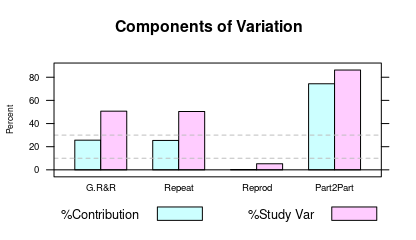
\includegraphics[scale = 1]{figures/graf1.png}
    \label{fig:compvar}

\end{figure}


Já na figura \ref{fig:r_maquina} podemos verificar a amplitude da amostra por operador. Observe que segundo a tabela \ref{tab:maquinas} temos quatro operadores diferentes e é exatamente isto que encontra-se disposto aqui. Cada ponto representa a diferença entre a maior e a menor leitura observada para cada uma das três medições realizadas em cada robô. Embora haja um certo padrão comportamental entre os quatro gráficos, valores muito distantes como o do robô 1 no operador 2 indicam a existência de dificuldades nesta medição. 
\begin{figure}[H]
	\caption{Amplitude da Amostra por Máquina}
	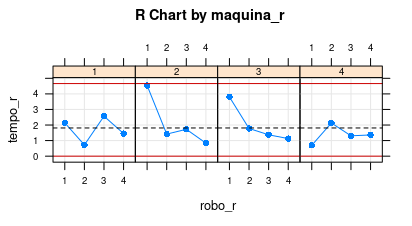
\includegraphics[]{figures/graf3.png}
	\label{fig:r_maquina}
\end{figure}


\begin{figure}[H]
	\centering
	\caption{Média da amostra por máquina}
	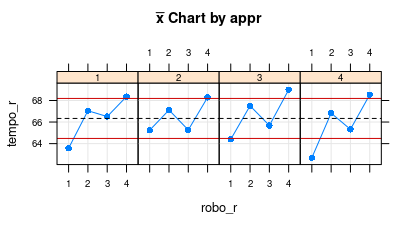
\includegraphics[scale = 1]{figures/graf5.png}
	\label{fig:graf5}
\end{figure}

Na Figura \ref{fig:graf5} é plotada a média das medições com o mesmo intuito do gráfico Amplitude de Amostra por Máquina. Mas neste caso a média é utilizada. Neste gráfico estão exibidas as médias do tempo para cada robô. Podemos observar que há um comportamento similar entre as máquinas 2 e 3, porém as máquinas 1 e 4 exibem médias diferentes do que se esperava para o
sistema.

Na seção \textit{tempo\_r by\ robo\_r} exibida na figura \ref{fig:tempo_robo} encontram-se distribuídas em torno do ponto central (média) as leituras efetuadas para cada robô, sendo traçada uma reta ligando estas médias. Pode-se notar que existem alguns pontos distantes do ponto central, o que pode significar um erro de medição, uma medição ruim ou errada.
\begin{figure}[H]
	\caption{Tempo por Robô}
	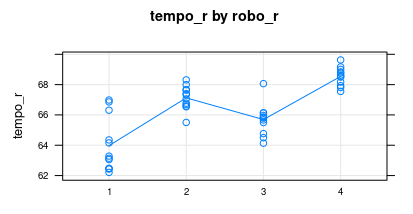
\includegraphics[]{figures/graf2.png}
	\label{fig:tempo_robo}
\end{figure}

\begin{figure}[H]
	\centering
	\caption{Tempo por máquina}
	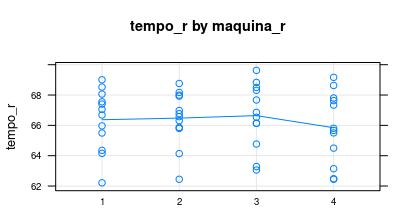
\includegraphics[scale = 1]{figures/graf4.png}
	\label{fig:graf4}
\end{figure}

Na Figura \ref{fig:graf4} cada um dos testes têm distribuídos em torno da linha azul central (a média) as leituras efetuadas. Note que as leituras se distribuem em torno das leituras em azul, o que significa que estão muito distantes do alvo o que representa um erro de leitura, uma leitura ruim ou errada. As medidas de tempo encontradas para cada um dos operadores encontram-se exibidos nesse gráfico, onde cada valor encontrado é representado por um círculo e uma reta passa por seus valores médios. Quanto menor o ângulo entre cada uma das máquinas melhor para o sistema, pois significa que não há grande diferença entre as capacidades de operação das máquinas.



\begin{figure}[H]
	\centering
	\caption{Média da amostra por máquina}
	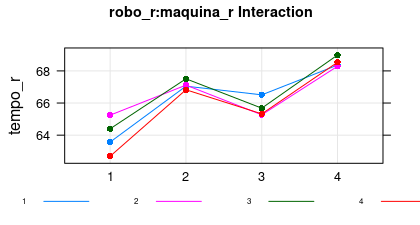
\includegraphics[scale = 1]{figures/graf6.png}
	\label{fig:graf6}
\end{figure}

Na seção \ref{fig:graf6} este gráfico apresenta uma junção dos gráficos exibidos em Média da amostra por máquina a fim de fazer uma comparação entre as médias encontradas para cada robô. É usado para checar se existe uma relação entre máquina e um robô específico. Caso alguma máquina tenha uma dificuldade com algum tipo de robô, será possível observar uma discrepância entre as linhas em determinado robô. No gráfico apresentado, verifica-se que há muita diferença entre cada máquina.

\section*{Conclusão}
O valor encontrado na porcentagem de variação do estudo classifica o sistema de medição como inaceitável. A não conformidade com o numero de categorias distintas também é um fator que contribui negativamente com os resultados encontrados. É uma solução possível a retomada dos dados e realização de novos testes.





%---------------------------------------------------------------------------------------
% Referências
	\cleardoublepage
	\titleformat{\chapter}[display]{\vspace*{-24pt}\ABNTEXchapterfont\large\bfseries}{\chaptertitlename\ \thechapter}{12pt}{\Large}
	\bibliography{bibliography}
% --------------------------------------------------------------------------
%Apêndices
	% \apendices
	% \justify
	% %
	% \chapter{\textit{Draft} do conceito (Vistas).}
	% \label{apend:draft}
	% \includepdf[pages={{},-}]{images/Desenho_tecnico_UGV-C_4vistas.pdf}
	% % \lipsum[1] % Comentar e adicionar apêndice aqui
	% %
	% \chapter{\textit{Draft} do conceito (Isométrica).}
	% \label{apend:draftiso}
	% \includepdf[pages={{},-}]{images/iso.pdf}
	% % \lipsum[1] % Comentar e adicionar apêndice aqui

	% \chapter{Desdobramento da Função Qualidade.}
	% \label{apend:qfd}
	% \includepdf[scale=1.64]{images/QFD.pdf}
	
	

% --------------------------------------------------------------------------
% Anexos                                                                     
	% \anexos
	% \justify
	% %
	% \chapter{Outro assunto importante}
	% \label{ann:relant}
	% %\includepdf[pages={{},-}]{annex/manisubanterioridade.pdf}
	% \lipsum[1] % Comentar e adicionar apêndice aqui
	% %
\end{document} 